\documentclass[11pt,letterpaper]{article}
\PassOptionsToPackage{hyphens}{url}
\usepackage[margin=.83in,top=.8in,bottom=.8in,headheight=15pt]{geometry}
\usepackage[T1]{fontenc}
\usepackage{lmodern,amsmath,amssymb,mathtools,bm,booktabs,array,graphicx,tikz}
\usetikzlibrary{arrows.meta,positioning,calc,decorations.pathreplacing,patterns}
\definecolor{ink}{HTML}{17344D}\definecolor{accent}{HTML}{087E8B}\definecolor{pale}{HTML}{EDF5F5}\definecolor{gold}{HTML}{AD6B19}
\providecommand{\dd}{\,\mathrm{d}}\providecommand{\R}{\mathbb{R}}
\providecommand{\E}{\mathbb{E}}\providecommand{\Var}{\operatorname{Var}}
\providecommand{\Cov}{\operatorname{Cov}}\providecommand{\diag}{\operatorname{diag}}
\providecommand{\norm}[1]{\left\lVert#1\right\rVert}
\providecommand{\abs}[1]{\left|#1\right|}
\usepackage{microtype,hyperref,fancyhdr,enumitem,amsthm,sectsty,needspace}
\allsectionsfont{\raggedright}
\hypersetup{colorlinks=true,linkcolor=ink,urlcolor=accent,pdfauthor={Zan Ahmad},pdftitle={A mixed chamber: differential equations and numerical stability / Lecture notes}}
\setlength{\parindent}{0pt}\setlength{\parskip}{6pt}\linespread{1.07}
\setlist{itemsep=3pt,topsep=4pt,leftmargin=*}
\emergencystretch=2em\clubpenalty=10000\widowpenalty=10000
\pagestyle{fancy}\fancyhf{}\fancyhead[L]{\small Mathematical Modeling}\fancyhead[R]{\small Lecture 3}
\fancyfoot[L]{\footnotesize Zan Ahmad}\fancyfoot[R]{\footnotesize\thepage}\renewcommand{\headrulewidth}{.3pt}
\newtheorem{proposition}{Proposition}\newtheorem{theorem}{Theorem}\newtheorem{lemma}{Lemma}
\theoremstyle{definition}\newtheorem{definition}{Definition}\newtheorem{example}{Example}
\numberwithin{equation}{section}
\begin{document}
{\small\scshape Mathematical Modeling\hfill Lecture 3}\par\medskip
{\raggedright\hyphenpenalty=10000\exhyphenpenalty=10000\LARGE\bfseries\color{ink} A mixed chamber: differential equations and numerical stability\par}\medskip
{\small Lecture notes}\par\bigskip
A conservation law becomes a dynamic model when removal depends on the amount currently stored. We derive a linear chamber equation from a mixing assumption, solve it exactly, and compare the continuous solution with forward Euler. Equilibrium, positivity, asymptotic stability, and accuracy are different properties. This example permits an algebraic analysis of each property, providing a basis for interpreting the computational plots.

\section{Concentration and the removal law}
\hypertarget{note-concentration-and-the-removal-law}{}\label{note:concentration-and-the-removal-law}
{\small \href{slides.html\#frame=mixing-and-mass-outflow\&step=1}{Slides for this section}}\par
Let a well-mixed chamber have fixed liquid volume $W$ and tracer mass $M(t)$ in mg. Its concentration is $c=M/W$. A volume outflow $Q$ removes tracer at rate $Qc=QM/W$. A balanced liquid inflow maintains $W$; denote its tracer contribution by the constant mass input $r\geq0$ in mg/min. With $k=Q/W\geq0$, conservation gives
\[
\boxed{\dot M=r-kM,\qquad M(0)=M_0\geq0.}
\]
The dimensions are $[M]=\mathrm{mg}$, $[r]=\mathrm{mg}/\mathrm{min}$, and $[k]=\mathrm{min}^{-1}$. If inflow concentration is $c_{\rm in}$, then $r=Qc_{\rm in}$. Mass input is not the same variable as liquid flow. The law assumes instantaneous mixing and fixed $Q/W$; the synthetic example is not a patient dosing model.

The same linear structure arises in a constant-compliance pressure balance with prescribed inflow. That analogy transfers solution methods, not parameter meanings or units. It connects this original chamber example with the circulation equations in the reading.
\section{Equilibrium and the integrating factor}
\hypertarget{note-equilibrium-and-the-integrating-factor}{}\label{note:equilibrium-and-the-integrating-factor}
{\small \href{slides.html\#frame=equilibrium-and-direction-of-motion\&step=1}{Slides for this section}}\par
For $k>0$, the equilibrium is $M_*=r/k$. Set $e=M-M_*$, so $\dot e=-ke$. Multiplying by $e^{kt}$ gives
\[
\frac{d}{dt}(e^{kt}e)=0,\qquad
\boxed{M(t)=M_*+(M_0-M_*)e^{-kt}.}
\]
Equivalently, $M(t)=e^{-kt}M_0+(1-e^{-kt})M_*$. The weights are nonnegative and sum to one. Hence the solution stays between $M_0$ and $M_*$, remains nonnegative, and approaches equilibrium monotonically. Its direction follows from $\dot M=k(M_*-M)$.

The relaxation time is $\tau=1/k$; after one $\tau$, departure from equilibrium is multiplied by $e^{-1}$. With $r>0$, set $m=M/M_*$ and $\theta=kt$ to obtain $dm/d\theta=1-m$. If $r=0$, decay remains valid without dividing by a zero equilibrium. If $k=0$, return to $\dot M=r$ and obtain $M=M_0+rt$. No finite attracting equilibrium exists when $k=0$ and $r>0$.

Near $k=0$, a numerically stable evaluation is $M_0e^{-kt}+r[-\operatorname{expm1}(-kt)/k]$, with the exact zero case handled separately. It avoids subtracting nearly equal values in $1-e^{-kt}$ and has limit $M_0+rt$.
\section{Forward Euler as a quadrature approximation}
\hypertarget{note-forward-euler-as-a-quadrature-approximation}{}\label{note:forward-euler-as-a-quadrature-approximation}
{\small \href{slides.html\#frame=euler-from-an-integral-balance\&step=1}{Slides for this section}}\par
The integral equation over one step is
\[
M(t_{n+1})-M(t_n)=\int_{t_n}^{t_{n+1}}[r-kM(s)]\,ds.
\]
Replacing the changing integrand by its old-state value gives, for $h=t_{n+1}-t_n$,
\[
\boxed{M_{n+1}=M_n+h(r-kM_n)=(1-kh)M_n+hr.}
\]
This is generally approximate because the removal rate changes within the step. In contrast, Meeting 1 integrated a prescribed constant rate exactly. Taylor expansion gives a local one-step error of order $h^2$ and generally a global error of order $h$ on a fixed finite interval.

For $r=2\ \mathrm{mg}/\mathrm{min}$ and $k=0.25\ \mathrm{min}^{-1}$, $M_*=8\ \mathrm{mg}$ and $\tau=4\ \mathrm{min}$. At $M=4\ \mathrm{mg}$, removal is $1\ \mathrm{mg}/\mathrm{min}$ and net input is $1\ \mathrm{mg}/\mathrm{min}$. A half-minute Euler step gives $4.5\ \mathrm{mg}$; the exact endpoint is $8-4e^{-0.125}\approx4.4700\ \mathrm{mg}$. Freezing the initially smaller removal overestimates the increase.
\begin{center}\begin{minipage}{.98\linewidth}\centering
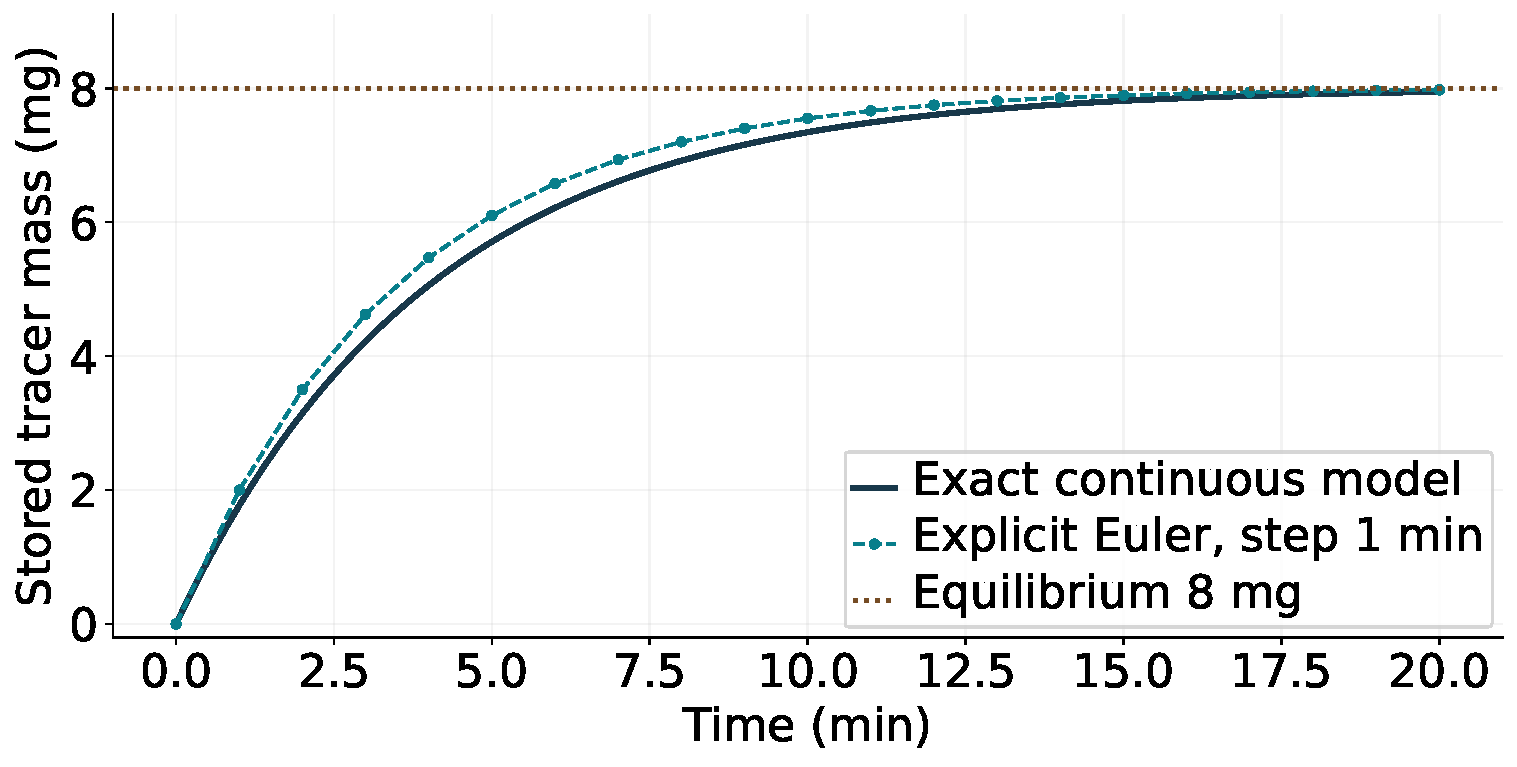
\includegraphics[width=.96\linewidth,height=.57\textheight,keepaspectratio]{presentation-figures/filling.pdf}\par\smallskip
{\small Synthetic chamber: input 2 mg/min, removal constant 0.25/min, initial mass 0. Euler uses a 1-minute step. Exact and numerical curves are distinct.}
\end{minipage}\end{center}
\section{The discrete amplification factor}
\hypertarget{note-the-discrete-amplification-factor}{}\label{note:the-discrete-amplification-factor}
{\small \href{slides.html\#frame=exact-discrete-recurrence\&step=1}{Slides for this section}}\par
On a uniform grid, substitute $e_n=M_n-M_*$ into Euler:
\[
e_{n+1}=(1-kh)e_n,\qquad
M_n=M_*+(M_0-M_*)(1-kh)^n.
\]
Put $a=1-kh$. For $0<kh<1$, departure decays without changing sign. At $kh=1$, Euler jumps to equilibrium in one step, unlike the exact finite-time response. For $1<kh<2$, departure alternates sign and decays. At $kh=2$ it alternates without decay; for $kh>2$ its magnitude grows.

Asymptotic stability requires $|a|<1$, or $0<kh<2$. A stronger condition guarantees nonnegative mass for all nonnegative old states and inputs:
\[
0\leq kh\leq1\quad\Longrightarrow\quad (1-kh)M_n+hr\geq0.
\]
With $r=0$ and $M_n>0$, $kh>1$ immediately produces a negative value, so the stronger bound is necessary for a guarantee over all such data. Stability alone does not establish positivity, monotonicity, or accuracy.
\section{Large-step trajectories and time refinement}
\hypertarget{note-large-step-trajectories-and-time-refinement}{}\label{note:large-step-trajectories-and-time-refinement}
{\small \href{slides.html\#frame=large-step-failure-modes-figure\&step=1}{Slides for this section}}\par
The baseline starts from $M_0=0$ with $h=1\ \mathrm{min}$, so $kh=0.25$. It rises toward $8\ \mathrm{mg}$ without crossing that value, but remains different from the exact curve. The two large-step experiments retain the same continuous equation and change only its discretization.

At $h=5\ \mathrm{min}$ the multiplier is $-0.25$, giving the initial sequence $0,10,7.5,8.125\ \mathrm{mg}$. This is stable but oscillatory. At $h=9\ \mathrm{min}$ the multiplier is $-1.25$, giving $0,18,-4.5,23.625\ \mathrm{mg}$: growing error and negative mass. Neither behavior belongs to the monotone exact solution.

At a fixed final time $T$, define $E(h)=|M_h(T)-M(T)|$. First-order convergence predicts $E(h)/E(h/2)\to2$ when the leading term dominates. Hold all physical inputs and the endpoint fixed. The code shortens a final partial step and uses its actual duration; comparing different endpoints would mix trajectory evolution with numerical error.
\begin{center}\begin{minipage}{.98\linewidth}\centering
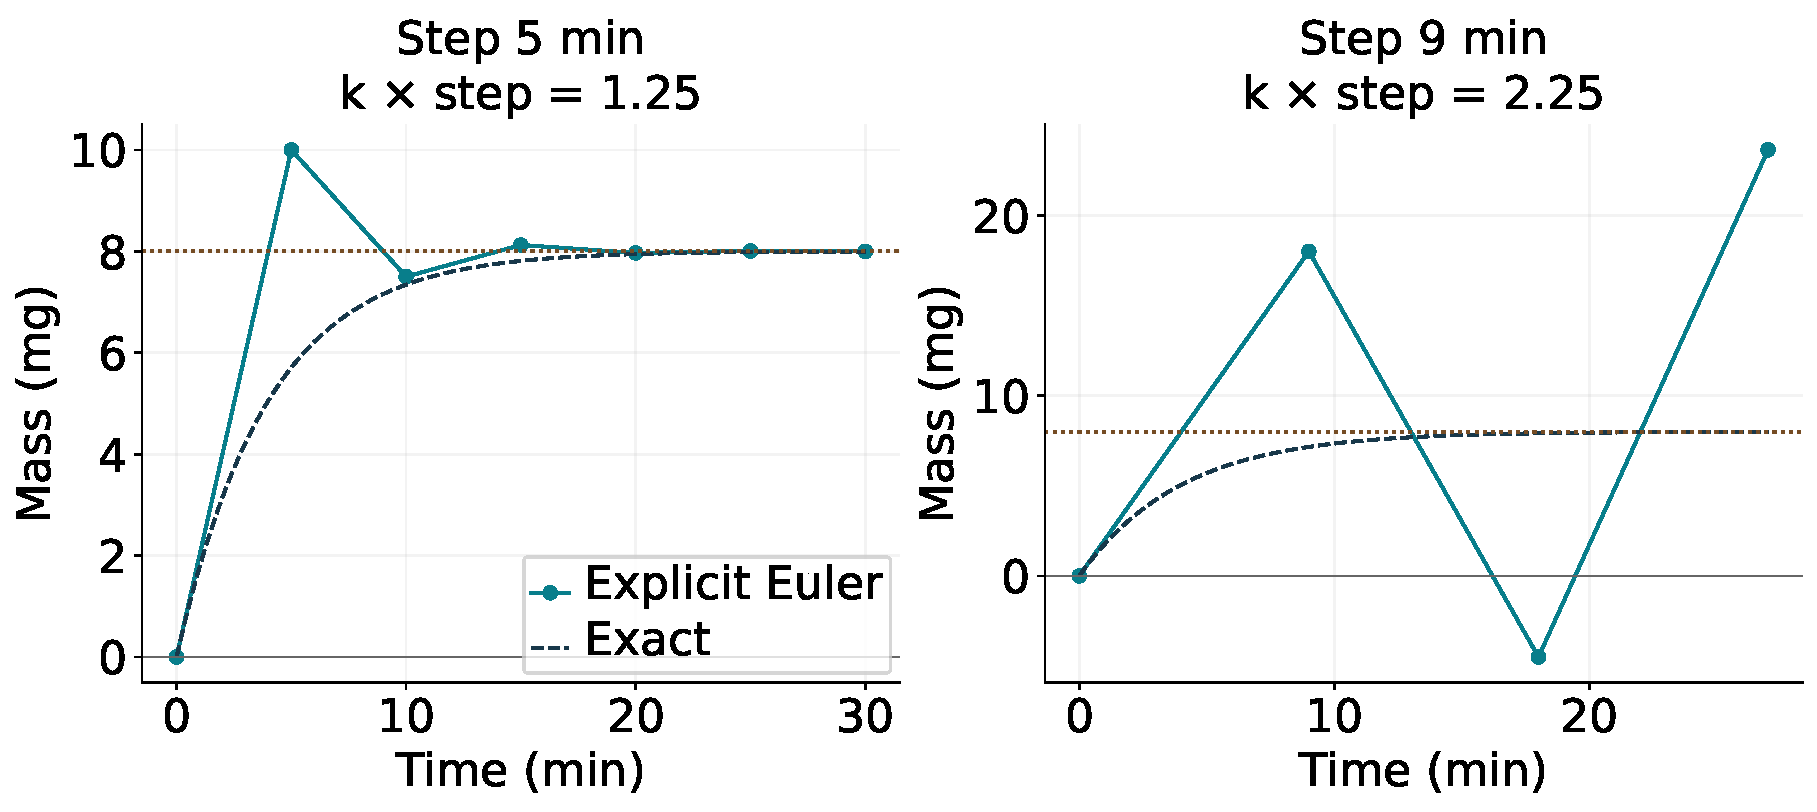
\includegraphics[width=.96\linewidth,height=.57\textheight,keepaspectratio]{presentation-figures/step-size.pdf}\par\smallskip
{\small A 5-minute step produces decaying oscillations; a 9-minute step produces growing error and negative mass. Both use the same continuous model.}
\end{minipage}\end{center}
\section{A conserved discrete account can conceal instability}
\hypertarget{note-a-conserved-discrete-account-can-conceal-instability}{}\label{note:a-conserved-discrete-account-can-conceal-instability}
{\small \href{slides.html\#frame=discrete-mass-budget\&step=1}{Slides for this section}}\par
Let $D_n$ be cumulative removed mass and update it with the same discrete transfer:
\[
D_{n+1}=D_n+hkM_n,\qquad D_0=0.
\]
Adding to the mass update yields $M_{n+1}+D_{n+1}=M_n+D_n+hr$, hence
\[
\boxed{M_n+D_n=M_0+rt_n.}
\]
This identity still holds for the oscillatory and negative trajectories. It checks the discrete bookkeeping, not the accuracy of the transfer approximation. Clipping negative mass would alter the account and conceal the failure.

Separate evidence is needed for separate claims. Check the invariant, exact equilibrium preservation, the $k=0$ linear limit, the $r=k=0$ constant limit, positivity at an admissible step, and refinement against the exact solution. Experimental validation then compares with independently measured tracer mass and can challenge mixing, constant volume, or proportional removal even when the numerical checks pass.
\bigskip
\section*{Exercises}
\par\noindent\begin{minipage}{\linewidth}
\subsection*{P1. A new chamber}
Use r=\allowbreak{}3 mg/min, k=\allowbreak{}0.5/min and initial mass 2 mg.

\textbf{a} Find equilibrium and the initial net rate.

\end{minipage}\par\medskip
\textbf{b} Take two explicit Euler steps of 0.5 minute.

\textbf{c} Is nonnegative mass guaranteed for this step and nonnegative input? Explain.

\par\noindent\begin{minipage}{\linewidth}
\subsection*{P2. The missing unit}
A student writes next\_mass =\allowbreak{} mass +\allowbreak{} rate\_in - k*mass.

\textbf{a} Explain the dimensional error.

\end{minipage}\par\medskip
\textbf{b} Repair the update and explain what must change if time is measured in seconds.

\par\noindent\begin{minipage}{\linewidth}
\subsection*{P3. Stable does not mean faithful}
Return to r=\allowbreak{}2 mg/min and k=\allowbreak{}.25/min with a non-equilibrium initial state.

\textbf{a} Classify full-step behavior for h=\allowbreak{}2, 6, 8 and 10 minutes.

\end{minipage}\par\medskip
\textbf{b} Which steps guarantee nonnegative mass for every nonnegative initial amount and input?

\textbf{c} A run passes conservation at h=\allowbreak{}10. Does that rescue it?

\par\noindent\begin{minipage}{\linewidth}
\subsection*{P4. A model versus an observation}
An experiment fills more slowly than both the exact curve and a refined numerical curve.

\textbf{a} Would another halving of a sufficiently small Euler step necessarily resolve the discrepancy?

\end{minipage}\par\medskip
\textbf{b} Name one assumption to test and one measurement that would help.

\section*{References}
\noindent\begin{minipage}{\linewidth}
Zan Ahmad, Fall 2024 HEART syllabus. PDF pages 1--2.

\end{minipage}\par\medskip
\noindent\begin{minipage}{\linewidth}
Hoppensteadt and Peskin, Modeling and Simulation in Medicine and the Life Sciences, second edition. Printed pages 39--41; PDF pages 52--54 in the supplied copy.

\end{minipage}\par\medskip
\end{document}
